%!TEX root = ../copatterns-thesis.tex
\chapter{Idris}
Idris is a general-purpose functional programming language with full dependent
types. To aid the presentation of our solution in the following chapters, this
chapter discusses the internal structure of the language implementation. Many of
the details of the implementation which are not covered here have been described
thoroughly by Brady\,\citep{BradyIdrisImpl13}.

% To understand how an implementation of guarded recursion could be realized in Idris, we must first understand the internal structure of the language. In this section we will first outline the overall structure of Idris and then dig into specific parts relevant to guarded recursion. This is not a thorough description of all of Idris's components, but rather an explanation of parts of the language. For more reading on this topic see Edwin Brady's .%todo: REF
\section{Overview}
%Idris -> Idris- -> TT -> Executable
\begin{figure}
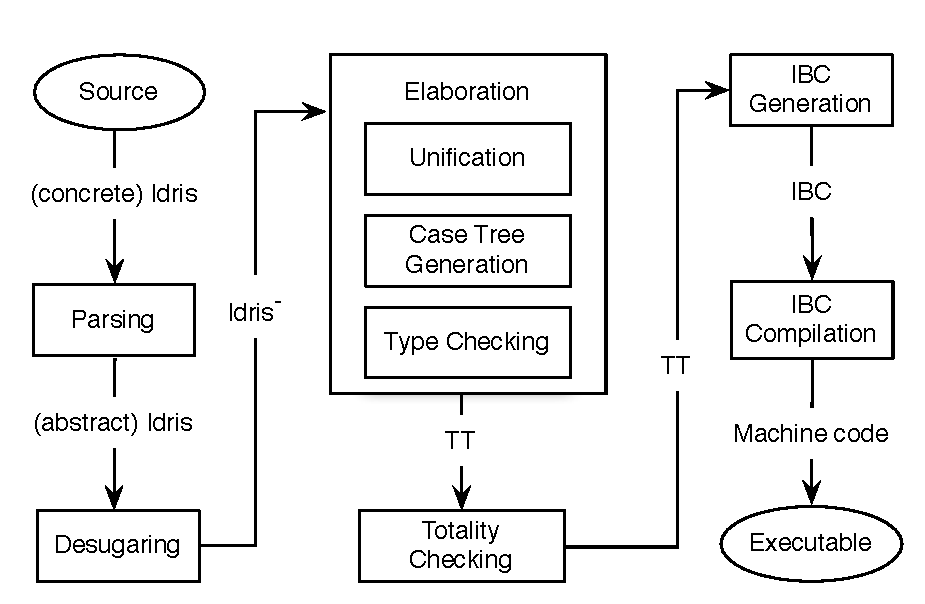
\includegraphics[scale=0.9]{figures/Idris-overview}
\caption{The phases of the Idris compiler. Phases are shown as rectangles, and
  each transition (arrow) is annotated with the input or output representation
  of a given phase. Ovals designate endpoints.}
\label{fig:idris-overview}
\end{figure}
\subsection{Language Representations}
\begin{itemize}
\item \textbf{(concrete) Idris}
The high-level language in which Idris programs are written.
\item \textbf{(abstract) Idris}
The abstract representation of the high-level Idris language.
\item \textbf{\IdrisM}
A (strict) subset of abstract Idris without any syntactic sugar. Do-notation and infix operators
are desugared, and implicit arguments are bound explicitly. Note that
\IdrisM and abstract Idris are essentially the same language, where the
syntactic sugar from abstract Idris is reduced to desugared terms.
\item \textbf{TT}
The core type theory, TT, is a dependently typed lambda calculus with inductive
types and pattern matching. TT only allows pattern matching on top-level values,
so all \texttt{case}-expressions are converted to top-level pattern matching
during elaboration. In TT, all terms are fully annotated with their types and
all implicit arguments are explicit.
\item \textbf{Raw}
A (raw) representation of TT terms without any type information on terms. This
representation is used for type reconstruction during type checking.
\item \textbf{IBC}
Idris Byte Code (IBC) is the bytecode representation of an Idris program.
\end{itemize}

\subsection{Phases of Compilation}
\begin{itemize}
\item \textbf{Source}
The source code of the program, given in concrete Idris syntax.
\item \textbf{Parsing}
The parser generates an abstract syntax tree (abstract Idris) from the source code.
\item \textbf{Desugaring}
 In the desugaring phase, abstract Idris is reduced to \IdrisM through
 desugaring.
\item \textbf{Elaboration}
Elaboration reduces \IdrisM terms to terms in the core calculus, TT. The
elaboration phase consists of several notable sub-phases:
\begin{itemize}
\item \textit{Unification}
Unification is the process of substituting holes for appropriate terms. It
enables elaboration to progress gradually by continually unifying holes with
terms, until a complete TT term has been built. Further details will be provided
in Section~\ref{sec:elaboration}.
\item \textit{Case Tree Generation}
For each function definition a case tree\,\citep{Augustsson:1985} is generated,
describing the structure of the top-level pattern matching. These case trees are
used for coverage checking during the totality checking phase.
\item \textit{Totality Checking}
During the totality checking phase, a totality analysis of each function
definition is performed. First, a coverage analysis determines whether the
function in question is covering (using the previously generated case
trees). Next, a termination analysis based on the size-change principle is
performed on supposedly terminating functions, while a productivity analysis is
performed on supposedly productive functions via the syntactic guardedness principle.
\item \textit{Type Checking}
All TT terms resulting from the previous steps of elaboration are type checked
at the end of elaboration to ensure that no ill-typed terms are
constructed. Type checking proceeds by converting TT terms to Raw terms, and
then reconstructing the type of each Raw term according to the typing
environment. If the reconstructed type is convertible with the annotated type of
the original TT term, type checking succeeds; otherwise, it fails.
\end{itemize}
\item \textbf{IBC Generation}
After successful elaboration, an Idris Byte Code representation is
generated by a script which is built up gradually during elaboration. 
\item \textbf{IBC Compilation}
During compilation, the IBC representation is reduced to a binary
representation.
\item \textbf{Executable}
The final executable generated by the compiler.
\end{itemize}
\subsection{Internal Representations}
\subsection{High-Level Abstract Syntax}
%PDecl/PTerm
%	Top level abstract syntax
%	Functions with multiple clauses are multiple Decls
\subsection{Dependently Typed Lambda Calculus}
%		TT
%			Dependently typed lambda calculus
%			Wrapped in case trees
%			Data and Type constructors??
\section{Elaboration}
\label{sec:elaboration}
\section{Totality checking}
%		Happens during and after elaboration
%			What happens when and why?
%		Coverage: Case Trees
%		Termination: Size Change
%			When are the graphs build?
%		Productivity: Syntactic Guardedness
\section{Type checking}
%??

%########
%% TT
% Alt er eksplicit
% Typeregler

%%% Type checking

%% Idris- / Desugaring
% Desugaring er en transformation fra Idris- til Idris-

%% Elaboration
% Hvorfor elaboration?
% Faser "smelter sammen" 
% Teknisk forklaring (tactic prover)

%% Totality checking
% Size-change termination
% Nuværende implementation af produktivitetschecker
% Totality er en forudsætning for type checking
% Erasure? (måske)


%########

%%% Local Variables:
%%% mode: latex
%%% TeX-master: "../copatterns-thesis"
%%% End:
